%% FullCourse_10Lecs -- Lecture 5, Topic 5.3: Actor-Critic + Applications + AlphaManager + Summary
%% Source: ./archive_pre_split/Lec05_RL_Nutshell.tex (sections 8-12)
%% Pass B: compared against
%%         ../../MiniCourse_8hr/Slides/Module2_DL_RL_Macro/M2_T3_RL_Basics.tex
%% Result: FullCourse is a strict superset of MiniCourse content for T3.
%%   MiniCourse Actor-Critic frames (Beyond Tabular, Architecture, Policy Gradient
%%   Theorem, A2C+PPO combined, RL Landscape, Recap) are all present here,
%%   typically split into more focused frames.
%% FullCourse-only frames (no MiniCourse counterpart):
%%   - Actor-Critic Algorithm (step-by-step pseudocode)
%%   - Why Actor-Critic for Economics?
%%   - DDPG: Deep Deterministic Policy Gradient
%%   - SAC: Soft Actor-Critic
%%   - Choosing an Algorithm: Summary
%%   - RL Breakthroughs: AlphaGo and Beyond
%%   - How AlphaGo Works: MCTS + RL (figure)
%%   - Monte Carlo Tree Search: Connection to Economics
%%   - Case Study: AlphaManager (3 frames: Offline RL, Policy Gradient & Ambiguity,
%%     Consistency and Extensions)  -- Campello, Cong, Zhou (2023)
%%   - Key Takeaways
%% NOTE: The AlphaManager case study (sec. 'Case Study') is FullCourse-only and
%%       unchanged in this pass.

%% Shared preamble for the FullCourse_10Lecs topic decks.
%%
%% Each topic .tex \input's this file, then defines its own \title, \date
%% override (if any), \graphicspath, and \begin{document}.
%%
%% Reconstructed verbatim from the inlined copy preserved in
%% Lec10_Case_Studies/Lec10_T8_Case6_DeepRamsey.tex (lines 23-190), which is
%% explicitly annotated there as "from ../shared_preamble.tex, copied verbatim".
%% Base preamble matches MiniCourse_8hr/Slides/shared_preamble.tex; this version
%% additionally provides \sectiondivider, the conceptbox/cautionbox/examplebox/
%% takeawaybox tcolorboxes, and \compacttables used across the split decks.

\documentclass[10pt,english,aspectratio=169]{beamer}

\usepackage{ae,aecompl}
\usepackage[T1]{fontenc}
\usepackage{textcomp}
\usepackage[utf8]{inputenc}
\usepackage{babel}
\usepackage{datetime2}

\setcounter{secnumdepth}{3}
\setcounter{tocdepth}{3}

\usepackage{amsmath, amssymb, amsthm, graphicx}
\usepackage{booktabs, multirow}
\usepackage{tikz}
\usepackage{pgfplots}
\pgfplotsset{compat=1.16}
\usepackage[most]{tcolorbox}
\tcbuselibrary{skins, breakable, theorems}
\usepackage{listings}
\usepackage{xcolor}

\lstset{
  basicstyle=\ttfamily\small,
  keywordstyle=\color{blue!80!black}\bfseries,
  commentstyle=\color{green!50!black}\itshape,
  stringstyle=\color{orange!80!black},
  backgroundcolor=\color{gray!8},
  frame=single,
  rulecolor=\color{gray!40},
  breaklines=true,
  showstringspaces=false,
  numbers=none,
}

\lstdefinestyle{pythonstyle}{
    language=Python,
    basicstyle=\ttfamily\footnotesize,
    keywordstyle=\color{blue!80!black}\bfseries,
    commentstyle=\color{green!50!black}\itshape,
    stringstyle=\color{orange!80!black},
    frame=single,
    breaklines=true,
    showstringspaces=false,
    numbers=left,
    numbersep=5pt,
    numberstyle=\tiny\color{gray},
    backgroundcolor=\color{gray!8},
    rulecolor=\color{gray!40}
}

\ifx\hypersetup\undefined
  \AtBeginDocument{%
    \hypersetup{bookmarks=false,breaklinks=true,pdfborder={0 0 0},colorlinks=true,
      linkcolor=DarkText,urlcolor=RedTitle}%
  }
\else
  \hypersetup{bookmarks=false,breaklinks=true,pdfborder={0 0 0},colorlinks=true,
    linkcolor=DarkText,urlcolor=RedTitle}%
\fi

\makeatletter
\newcommand\makebeamertitle{%
  \begin{frame}[plain]
    \vspace*{1.0cm}
    \centering
    {\usebeamerfont{title}\usebeamercolor[fg]{title}\inserttitle\par}
    \vspace{1.0cm}
    {\usebeamerfont{author}\usebeamercolor[fg]{author}\insertauthor\par}
    \vspace{0.2cm}
    {\usebeamerfont{date}\usebeamercolor[fg]{date}\insertdate\par}
  \end{frame}}%
\AtBeginDocument{%
  \let\origtableofcontents=\tableofcontents
  \def\tableofcontents{\@ifnextchar[{\origtableofcontents}{\gobbletableofcontents}}
  \def\gobbletableofcontents#1{\origtableofcontents}%
}

\usetheme{metropolis}
\usefonttheme{professionalfonts}

\definecolor{LightGray}{RGB}{230,230,230}
\definecolor{RedTitle}{RGB}{0,0,200}
\definecolor{VeryLightGray}{RGB}{245,245,245}
\definecolor{DarkText}{RGB}{0,0,0}

\setbeamercolor{background canvas}{bg=white}
\setbeamercolor{title}{fg=RedTitle}
\setbeamercolor{author}{fg=DarkText}
\setbeamercolor{date}{fg=DarkText}
\setbeamercolor{frametitle}{bg=VeryLightGray,fg=DarkText}
\setbeamercolor{normal text}{fg=DarkText}
\setbeamerfont{title}{size=\large}

\setbeamersize{text margin left=5mm, text margin right=5mm}
\addtobeamertemplate{frametitle}{}{\vspace{-0.5em}}
\newcommand{\reducevspace}{\vspace{-0.5cm}}

% Shared section divider and box styles for split topic decks.
\newcommand{\sectiondivider}[2]{%
\begin{frame}[plain,noframenumbering]
\begin{center}
\vfill
{\Large\textbf{#1}\par}
\vspace{0.35cm}
{\normalsize #2\par}
\vfill
\end{center}
\end{frame}
}

\newtcolorbox{conceptbox}[1][]{
  colback=blue!3,
  colframe=RedTitle!55,
  boxrule=0.35mm,
  arc=1mm,
  left=2mm,
  right=2mm,
  top=1mm,
  bottom=1mm,
  #1
}
\newtcolorbox{cautionbox}[1][]{
  colback=red!3,
  colframe=red!50!black,
  boxrule=0.35mm,
  arc=1mm,
  left=2mm,
  right=2mm,
  top=1mm,
  bottom=1mm,
  #1
}
\newtcolorbox{examplebox}[1][]{
  colback=green!3,
  colframe=green!45!black,
  boxrule=0.35mm,
  arc=1mm,
  left=2mm,
  right=2mm,
  top=1mm,
  bottom=1mm,
  #1
}
\newtcolorbox{takeawaybox}[1][]{
  colback=VeryLightGray,
  colframe=RedTitle!55,
  boxrule=0.35mm,
  arc=1mm,
  left=2mm,
  right=2mm,
  top=1mm,
  bottom=1mm,
  #1
}
\newcommand{\compacttables}{\renewcommand{\arraystretch}{1.15}}

\setbeamertemplate{navigation symbols}{}
\setbeamertemplate{footline}{%
  \hfill%
  \usebeamercolor[fg]{page number in head/foot}%
  \usebeamerfont{page number in head/foot}%
  \insertframenumber\,/\,\inserttotalframenumber\kern1em\vskip2pt%
}

\makeatother

\author{Zhigang Feng}
% "date with time": compile timestamp so each build is identifiable.
\date{\today\ \DTMcurrenttime}


\graphicspath{{./pic/}{../../MiniCourse_8hr/Slides/Module2_DL_RL_Macro/pic/}{../}}

% Suppress the redundant auto-generated metropolis section page; the
% \sectiondivider frames below are the dividers we keep.
\metroset{sectionpage=none}
\usetikzlibrary{positioning,arrows.meta,shapes,calc}
%% Lec05 shared MAP slide: "one backbone, three acts" recurring diagram.
%% Input this file AFTER ../shared_preamble.tex (needs RedTitle, VeryLightGray,
%% DarkText) and AFTER \usetikzlibrary{positioning,arrows.meta,shapes,calc}.
%% Call \LecFiveMap{k} inside a frame, where k in {1,2,3} highlights the current
%% act ("you are here") and k = 0 renders the closing reprise with all three
%% acts checked green (used by T3's closing synthesis frame).
%% Filename deliberately does NOT match the build glob Lec*_T*.tex, so the build
%% script never tries to compile it standalone.
%%
%% The three acts double as the lecture's spine: MODEL -> SAMPLE -> SCALE, i.e.
%% the three ways RL fills the Bellman expectation --- full backup (needs P,R),
%% sample backup (model-free), then sampled + function-approximated (deep RL).

\newcommand{\LecFiveMap}[1]{%
% Precompute per-box style selectors; TikZ option lists are comma-split before
% TeX conditionals run, so \ifnum must not sit inside a [...] options list.
\ifnum#1=0
  \tikzset{lmapa/.style={lmapdone}, lmapb/.style={lmapdone},
           lmapc/.style={lmapdone}}%
\else
  \tikzset{lmapa/.style={}, lmapb/.style={}, lmapc/.style={}}%
  \ifnum#1=1 \tikzset{lmapa/.style={lmapcur}}\fi
  \ifnum#1=2 \tikzset{lmapb/.style={lmapcur}}\fi
  \ifnum#1=3 \tikzset{lmapc/.style={lmapcur}}\fi
\fi
\begin{center}
\begin{tikzpicture}[
    act/.style={rectangle, rounded corners, draw=black!60, fill=VeryLightGray,
        minimum width=3.4cm, minimum height=1.0cm, text width=3.25cm,
        align=center, font=\small, text=DarkText},
    lmapcur/.style={draw=RedTitle, very thick, fill=orange!20},
    lmapdone/.style={draw=green!45!black, thick, fill=green!10},
    q/.style={font=\tiny\itshape, text width=3.4cm, align=center, text=black!70},
    barlab/.style={font=\tiny\bfseries, text=black!65},
    sat/.style={rectangle, rounded corners, draw=black!45, dashed, fill=white,
        text width=4.3cm, align=center, font=\tiny, text=black!70,
        minimum height=0.5cm},
    arr/.style={-{Stealth[length=2.4mm]}, thick, gray!60}
]
    % --- three act boxes ---
    \node[act, lmapa] (a1) at (0,0)
        {\textbf{5.1\ \ MODEL}\\[1pt] \tiny MDP \& the DP bridge};
    \node[act, lmapb] (a2) at (4.5,0)
        {\textbf{5.2\ \ SAMPLE}\\[1pt] \tiny MC $\cdot$ TD $\cdot$ Q-learning};
    \node[act, lmapc] (a3) at (9.0,0)
        {\textbf{5.3\ \ SCALE}\\[1pt] \tiny actor--critic $\cdot$ deep RL};
    \draw[arr] (a1) -- (a2);
    \draw[arr] (a2) -- (a3);
    % --- the student question each act answers ---
    \node[q] at (0,-0.98)   {what is RL, and how does it\\ relate to the DP I know?};
    \node[q] at (4.5,-0.98) {how do I learn a policy with\\ no model of the world?};
    \node[q] at (9.0,-0.98) {how does it scale --- and\\ where has it worked?};
    % --- "you are here" marker above the current act ---
    \ifnum#1=1 \node[font=\scriptsize\bfseries, text=RedTitle] at (0,1.02)
        {you are here\ $\blacktriangledown$};\fi
    \ifnum#1=2 \node[font=\scriptsize\bfseries, text=RedTitle] at (4.5,1.02)
        {you are here\ $\blacktriangledown$};\fi
    \ifnum#1=3 \node[font=\scriptsize\bfseries, text=RedTitle] at (9.0,1.02)
        {you are here\ $\blacktriangledown$};\fi
    \ifnum#1=0 \node[font=\scriptsize\bfseries, text=green!45!black] at (4.5,1.02)
        {all three acts complete};\fi
    % --- bottom band: the backup taxonomy (the technical spine of the lecture) ---
    \fill[blue!10]   (-1.6,-1.78) rectangle (1.6,-1.45);
    \fill[green!12]  (2.9,-1.78)  rectangle (6.1,-1.45);
    \fill[orange!16] (7.4,-1.78)  rectangle (10.6,-1.45);
    \node[barlab] at (0,-1.615)   {FULL BACKUP\ (needs $P,R$)};
    \node[barlab] at (4.5,-1.615) {SAMPLE BACKUP\ (model-free)};
    \node[barlab] at (9.0,-1.615) {SAMPLED $+$ APPROXIMATED};
    % --- dashed satellites: where this lecture sits in the course flow ---
    \node[sat] at (0,-2.45)
        {\textit{upstream:} Lec02 (RL = 3rd ML pillar), Lec04 T2 (RL as a Bellman solver)};
    \node[sat] at (9.0,-2.45)
        {\textit{downstream:} Lec06 --- HA models at scale (Aiyagari, Krusell--Smith, DeepHAM)};
\end{tikzpicture}
\end{center}
}


\title[AI for Econ Research]{AI for Economic Research: Dynamic Models, Language, and Agents\\
Lecture 5.3: Actor-Critic Methods, Applications, and the AlphaManager Case}
\author{Zhigang Feng}
\date{\today\ \DTMcurrenttime}

\begin{document}

\makebeamertitle

%=============================================================================
\begin{frame}{Lecture 5 in One Map --- Act 5.3}
\textbf{Acts 5.1--5.2 executed departure \#1 (sample the backup) --- but still store values in \emph{tables}. This act executes departure \#2: \emph{approximate the function} --- neural networks for $V$, $Q$, $\pi$ --- and shows where the recipe has worked.}

\LecFiveMap{3}

\vspace{0.05cm}
\footnotesize\textit{The internal flow of this act: tables $\to$ \textbf{function approximation} (the deadly triad, DQN) $\to$ \textbf{actor--critic} and the policy-gradient family (A2C, DDPG, PPO, SAC) $\to$ \textbf{applications} (AlphaGo, RLHF) $\to$ two economic cases: \textbf{AlphaManager} (corporate finance) and \textbf{Krusell--Smith} (heterogeneous agents) $\to$ synthesis and the hand-off to Lec06.}
\end{frame}

%=============================================================================
\section{Actor-Critic Methods}

\sectiondivider{Actor--Critic Methods}{From tables to neural networks --- and how to make them stable}

\begin{frame}{Motivation: Beyond Tabular Methods}
    \textit{Recall:} Lec04 T2 previewed actor-critic as a Bellman solver; here we formalize it as the policy-gradient family with convergence theory and the A2C / A3C / PPO / DDPG / SAC variants.

    \vspace{0.2cm}
    \textbf{Tabular RL:}
    \begin{itemize}
        \item Stores a value for each \emph{discrete} state (or state--action) pair.
        \item Infeasible in \textbf{large or continuous} state spaces.
    \end{itemize}

    \vspace{0.3cm}
    \textbf{Function Approximation:}
    \begin{itemize}
        \item Replace tables with \textbf{parameterized models} (e.g., neural networks).
        \item Generalize from observed states to unseen states.
    \end{itemize}

    \vspace{0.3cm}
    \textbf{Continuous Action Spaces:}
    \begin{itemize}
        \item Economic decisions are typically \textbf{continuous}: how much to consume, invest, price.
        \item Cannot enumerate all actions $\Rightarrow$ need a \textbf{continuous policy} $\pi_\theta(a|s)$.
        \item Actor-critic methods handle this naturally.
    \end{itemize}
\end{frame}

% NEW: function approximation + semi-gradient TD + deadly triad (book Ch13 §3.1)
\begin{frame}{From Tables to Function Approximation}
\textbf{Replace the table} $V(s)$ / $Q(s,a)$ \textbf{with a parameterized function} $V_w(s)$ --- linear $w^\top\phi(s)$, then neural.
\begin{itemize}
  \item \textbf{Semi-gradient TD(0):} $w \gets w + \alpha\,\delta_t\,\nabla_w V_w(s_t)$, with the bootstrap target held fixed.
  \item \textbf{Why:} parameters \textbf{generalize} across states; storage grows with dimension, not as $m^d$ --- though this \emph{mitigates}, not \emph{eradicates}, the curse.
  \item \textbf{Shared with DP:} the same projection idea economists already use (Chebyshev, splines); the neural net is its nonlinear generalization.
\end{itemize}
\vspace{0.1cm}
\begin{cautionbox}
\textbf{The deadly triad} (Sutton \& Barto): \textbf{off-policy} $+$ \textbf{function approximation} $+$ \textbf{bootstrapping}, together, can \emph{diverge} --- one overestimate feeds its own target and spreads via generalization. Tabular RL never had this; the classical contraction guarantees no longer apply.
\end{cautionbox}
\end{frame}

% NEW: DQN as engineering patches for the triad (book Ch13 §3.2)
\begin{frame}{DQN: Making Neural Q-Learning Work}
\hfill\footnotesize{Mnih et al.\ (2015), \emph{Nature}, ``Human-level control through deep RL''}\normalsize

Plugging a neural net $Q_\theta(s,a)$ straight into Q-learning \textbf{ignites the triad} (off-policy $+$ NN $+$ bootstrap) --- it oscillates or diverges. \textbf{DQN} stabilizes it with two engineering patches:
\begin{itemize}
  \item \textbf{Experience replay:} store transitions in a buffer, sample mini-batches --- breaks temporal correlation, restores (approx.) i.i.d.\ for SGD, reuses data.
  \item \textbf{Target network} $\theta^-$: a \emph{lagged} copy used in the target $y_t = r_{t+1} + \gamma \max_{a'} Q_{\theta^-}(s_{t+1},a')$, synced every $C$ steps --- freezes the bootstrap loop so the net fits a \emph{stable} target.
\end{itemize}
\vspace{0.1cm}
\footnotesize\textit{Patches, not a principled fix --- DQN still needs careful tuning. And $\max_{a'}$ needs enumerable actions, which breaks for continuous controls $\Rightarrow$ the policy-gradient / actor-critic route next.}\normalsize
\end{frame}

\begin{frame}{Actor-Critic: The Architecture}
    Two sets of parameters, trained jointly:

    \vspace{0.3cm}
    \textbf{Actor (Policy $\pi_\theta$):}
    \begin{itemize}
        \item Parameterized by $\theta$ (e.g., neural network weights).
        \item Produces actions: $a \sim \pi_\theta(a|s)$.
        \item Updated via \textbf{policy gradient}.
    \end{itemize}

    \vspace{0.3cm}
    \textbf{Critic (Value Function $V_\phi$ or $Q_\phi$):}
    \begin{itemize}
        \item Parameterized by $\phi$.
        \item Estimates expected return: $V^\pi(s;\phi)$ or $Q^\pi(s,a;\phi)$.
        \item Provides feedback (``critique'') to guide the actor.
        \item Updated via \textbf{TD learning}.
    \end{itemize}

    \vspace{0.3cm}
    \textbf{Why combine?} Policy methods handle continuous actions; value methods reduce variance. Actor-critic merges both for efficient learning.
\end{frame}


\begin{frame}{Policy Gradient Theorem}
    \hfill\footnotesize{Sutton, McAllester, Singh \& Mansour, \emph{NIPS} 1999 (proc.\ 2000)}\normalsize

    \textbf{Objective:}
    $J(\theta) = \mathbb{E}_{\pi_\theta}\!\left[\sum_{t=0}^{\infty} \gamma^t r_t\right]$.

    \vspace{0.2cm}
    \textbf{Policy Gradient Theorem:}
    \[
      \nabla_\theta J(\theta)
      =
      \mathbb{E}_{s \sim d^{\pi_\theta},\, a \sim \pi_\theta}
      \Bigl[
         \nabla_\theta \log\pi_\theta(a | s)\,Q^{\pi_\theta}(s,a)
      \Bigr].
    \]

    \begin{itemize}
        \item The \textbf{log-derivative trick}: we only differentiate $\log \pi_\theta(a|s)$.
        \item Multiplying by $Q^{\pi_\theta}(s,a)$ emphasizes actions with higher returns.
        \item In practice, the \textbf{critic} approximates $Q$ (or $V$) with parameters $\phi$.
    \end{itemize}

    \vspace{0.3cm}
    \textbf{Variance reduction:} Replace $Q^\pi(s,a)$ with the \textbf{advantage}:
    \[
    A^\pi(s,a) = Q^\pi(s,a) - V^\pi(s).
    \]
    Subtracting the baseline $V^\pi(s)$ keeps the estimate unbiased but lowers variance.
\end{frame}


% NEW: REINFORCE, score function, masked softmax (book Ch13 §4.1)
\begin{frame}{REINFORCE: the Score-Function Estimator}
\textbf{The environment drops out.} Since $\nabla_\theta \log p_\theta(\tau) = \sum_t \nabla_\theta \log \pi_\theta(a_t|s_t)$, the transition terms \emph{vanish} --- the policy gradient is \textbf{model-free}:
\[
  \nabla_\theta J(\theta) = \mathbb{E}\Bigl[\textstyle\sum_t \nabla_\theta \log \pi_\theta(a_t|s_t)\,\bigl(G_t - b(s_t)\bigr)\Bigr].
\]
\begin{itemize}
  \item \textbf{REINFORCE} (Williams 1992): sample a trajectory, ascend this gradient. Unbiased, but \textbf{high variance}.
  \item \textbf{Baseline} $b(s_t)=V(s_t)$: keeps the gradient unbiased while cutting variance --- exactly the \textbf{control-variate} trick from GMM. The bracket becomes the \textbf{advantage} $A_t \approx Q-V$.
  \item \textbf{Constraints:} a \textbf{masked softmax} sends infeasible-action logits to $-\infty$, so $\pi_\theta$ respects the budget set.
\end{itemize}
\end{frame}

% FullCourse-only: explicit actor-critic pseudocode (Mini stops at the architecture)
\begin{frame}{Actor-Critic Algorithm}
\textbf{At each time step:}
\begin{enumerate}
    \item \textbf{Actor} selects action: $a_t \sim \pi_\theta(\cdot | s_t)$.
    \item Environment returns $(r_{t+1}, s_{t+1})$.
    \item \textbf{Critic update} (TD learning on $\phi$):
    \[
        \delta_t = r_{t+1} + \gamma V(s_{t+1};\phi) - V(s_t;\phi)
    \]
    \[
       \phi \gets \phi + \alpha\,\delta_t\,\nabla_\phi V(s_t;\phi)
    \]
    \item \textbf{Actor update} (policy gradient on $\theta$):
    \[
       \theta \gets \theta + \beta\,\delta_t\,\nabla_\theta \log \pi_\theta(a_t | s_t)
    \]
\end{enumerate}

\vspace{0.2cm}
\textbf{Intuition:}
\begin{itemize}
    \item $\delta_t > 0$: outcome was \textbf{better} than expected $\Rightarrow$ increase probability of $a_t$.
    \item $\delta_t < 0$: outcome was \textbf{worse} than expected $\Rightarrow$ decrease probability of $a_t$.
\end{itemize}
\end{frame}


% FullCourse-only: explicit "why AC for econ" frame
\begin{frame}{Why Actor-Critic for Economics?}
    \textbf{Large / Continuous State Spaces:}
    \begin{itemize}
        \item Capital stocks, prices, wealth distributions --- high-dimensional and continuous.
        \item Function approximation with neural networks is essential.
    \end{itemize}

    \vspace{0.2cm}
    \textbf{Continuous Action Spaces:}
    \begin{itemize}
        \item Monetary policy rates, consumption levels, investment amounts.
        \item Actor-critic handles continuous actions via a learned policy $\pi_\theta(a|s)$.
    \end{itemize}

    \vspace{0.2cm}
    \textbf{Efficiency and Stability:}
    \begin{itemize}
        \item Critic reduces variance in policy updates.
        \item More data-efficient than pure policy gradient or pure value-based methods.
    \end{itemize}

    \vspace{0.2cm}
    \textbf{Already seen in Lec04:} The simple actor-critic applied to the optimal growth model (policy NN + value NN trained jointly).
\end{frame}


% NEW: five-algorithm ladder + AC = online two-step estimation (book Ch13 §5.3)
\begin{frame}{One Ladder: MC Control $\to$ SARSA $\to$ Q $\to$ REINFORCE $\to$ AC}
\small
\begin{enumerate}
  \item \textbf{MC control} --- full-return evaluation; high variance, needs episode end.
  \item $+$ one-step bootstrap $\Rightarrow$ \textbf{SARSA} (on-policy TD control).
  \item $+$ $\max$ / off-policy $\Rightarrow$ \textbf{Q-learning} (targets the optimum).
  \item $+$ direct policy gradient $\Rightarrow$ \textbf{REINFORCE} (continuous actions; high variance).
  \item $+$ a TD critic as the baseline $\Rightarrow$ \textbf{Actor-Critic} (low-variance gradient).
\end{enumerate}
\normalsize
\vspace{0.1cm}
\begin{conceptbox}
\textbf{Actor-Critic $\approx$ online two-step estimation.} The \textbf{critic} is the first-stage \emph{nuisance} parameter (the value); the \textbf{actor}, the second-stage structural parameter (the policy) --- the rolling version of the two-step M-estimator economists know (Newey--McFadden 1994), interleaved rather than waiting for stage one to converge.
\end{conceptbox}
\end{frame}

%=============================================================================
\section{Advanced Actor-Critic Algorithms}

\sectiondivider{Advanced Actor--Critic Algorithms}{A2C/A3C, DDPG, PPO, SAC --- and how to choose among them}

\begin{frame}{A2C / A3C: Advantage Actor-Critic}
    \hfill\footnotesize{A3C: Mnih et al.\ (2016), \emph{ICML}, ``Asynchronous Methods for Deep RL''; A2C: OpenAI Baselines (2017)}\normalsize

    \textbf{Key idea:} Use the advantage function $A_t = r_t + \gamma V(s_{t+1}) - V(s_t)$
    in the policy gradient:
    \[
      \nabla_\theta J(\theta) \approx \sum_t A_t \, \nabla_\theta \log \pi_\theta(a_t | s_t).
    \]

    \vspace{0.3cm}
    \textbf{A3C (Asynchronous)} --- the original method (Mnih et al.\ 2016):
    \begin{itemize}
        \item Multiple \textbf{workers} run parallel environment instances.
        \item Workers update \textbf{asynchronously} --- faster but gradients may become stale.
    \end{itemize}

    \vspace{0.2cm}
    \textbf{A2C (Synchronous)} --- the synchronous variant popularized by OpenAI Baselines (2017):
    \begin{itemize}
        \item Workers synchronously send gradients to a central learner --- simpler and often more stable.
    \end{itemize}

    \vspace{0.3cm}
    \textbf{For economists:} parallel workers $=$ running multiple economy simulations simultaneously, each feeding back to improve a shared policy.
\end{frame}


% FullCourse-only: DDPG dedicated frame (Mini bundles modern AC variants briefly)
\begin{frame}{DDPG: Deep Deterministic Policy Gradient}
    \hfill\footnotesize{Lillicrap et al.\ (2016), \emph{ICLR}, ``Continuous Control with Deep RL''}\normalsize

    \textbf{For continuous action spaces with a deterministic policy $\mu_\theta(s)$:}
    \begin{itemize}
        \item \textbf{Actor:} $a = \mu_\theta(s)$ --- deterministic mapping from state to action.
        \item \textbf{Critic:} $Q_\phi(s,a)$ --- approximates expected return for $(s,a)$.
    \end{itemize}

    \vspace{0.3cm}
    \textbf{Policy gradient (chain rule through the critic):}
    \[
      \nabla_\theta J \approx \frac{1}{N}\sum_i
      \nabla_a Q_\phi(s_i,a)\big|_{a=\mu_\theta(s_i)}
      \cdot \nabla_\theta \mu_\theta(s_i).
    \]

    \vspace{0.2cm}
    \textbf{Exploration:} Add noise to actions: $a_t = \mu_\theta(s_t) + \text{noise}$.

    \vspace{0.3cm}
    \textbf{Economic applications:}
    \begin{itemize}
        \item Continuous portfolio allocation adjustments.
        \item Optimal consumption/investment with continuous controls.
    \end{itemize}
\end{frame}


\begin{frame}{PPO: Proximal Policy Optimization}
    \hfill\footnotesize{Schulman, Wolski, Dhariwal, Radford \& Klimov (2017), arXiv:1707.06347}\normalsize

    \textbf{Problem:} Large policy updates can destabilize learning.

    \vspace{0.2cm}
    \textbf{Solution:} Clip the policy ratio to prevent drastic changes:
    \[
      L^{\text{clip}}(\theta) = \mathbb{E}_t\!\left[
        \min\!\left(
          \frac{\pi_\theta(a_t|s_t)}{\pi_{\theta_{\text{old}}}(a_t|s_t)} A_t,\;
          \text{clip}\!\left(\frac{\pi_\theta}{\pi_{\theta_{\text{old}}}},\, 1{-}\epsilon,\, 1{+}\epsilon\right) A_t
        \right)
      \right].
    \]

    \begin{itemize}
        \item $\epsilon \approx 0.2$: bounds how much the policy can change per update.
        \item If $A_t > 0$ (good action): increase its probability, but not too much.
        \item If $A_t < 0$ (bad action): decrease its probability, but not too much.
    \end{itemize}

    \vspace{0.3cm}
    \textbf{Why popular?} Simple, stable, good performance across diverse tasks. Widely used in training LLMs via RLHF (Reinforcement Learning from Human Feedback).
\end{frame}


% FullCourse-only: SAC + entropy regularization (Mini only mentions SAC briefly)
\begin{frame}{SAC: Soft Actor-Critic}
    \hfill\footnotesize{Haarnoja, Zhou, Abbeel \& Levine (2018), \emph{ICML}, ``Soft Actor-Critic''}\normalsize

    \textbf{Key innovation:} Add \textbf{entropy regularization} to the objective.
    \[
      J_{\text{SAC}} = \mathbb{E}\!\left[\sum_t \gamma^t\bigl(r_t + \alpha \,\mathcal{H}(\pi(\cdot|s_t))\bigr)\right],
    \]
    where $\mathcal{H}(\pi) = -\sum_a \pi(a|s)\log\pi(a|s)$ measures policy ``spread.''

    \vspace{0.3cm}
    \begin{itemize}
        \item $\alpha$ large $\Rightarrow$ more exploration (high-entropy policy).
        \item $\alpha$ small $\Rightarrow$ more exploitation (near-deterministic).
        \item Prevents premature convergence to local optima.
    \end{itemize}

    \vspace{0.3cm}
    \textbf{Practical features:} Twin Q-networks (reduce overestimation), soft target updates (stability), stochastic policy (reparameterization trick).

    \vspace{0.2cm}
    \textbf{When to use:} Uncertain environments requiring robust exploration.
\end{frame}


% FullCourse-only: algorithm selection summary table for economists
\begin{frame}{Choosing an Algorithm: Summary}
    \small
    \begin{center}
    \begin{tabular}{llll}
        \toprule
        \textbf{Algorithm} & \textbf{Key Feature} & \textbf{Action Space} & \textbf{Best For} \\
        \midrule
        Q-Learning & Off-policy, tabular & Discrete & Small problems \\
        A2C/A3C & Advantage + parallel & Both & Parallel simulations \\
        DDPG & Deterministic policy & Continuous & Single best action \\
        PPO & Clipped updates & Both & Stable improvements \\
        SAC & Entropy regularization & Continuous & Robust exploration \\
        \bottomrule
    \end{tabular}
    \end{center}

    \vspace{0.3cm}
    \normalsize
    \textbf{For economists solving macro models:}
    \begin{itemize}
        \item \textbf{Known model, continuous controls:} Actor-critic (DDPG or PPO).
        \item \textbf{Unknown environment, need exploration:} SAC or PPO.
        \item \textbf{Discrete actions, small state space:} Q-learning suffices.
        \item \textbf{Training LLMs (RLHF):} PPO is the standard.
    \end{itemize}
\end{frame}


% NEW: honest deep-RL challenges (book Ch13 §6.3)
\begin{frame}{Deep RL in Practice: Four Honest Challenges}
\begin{enumerate}
  \item \textbf{Sample inefficiency:} $10^5$--$10^7$ environment steps --- vs.\ $\sim$200 quarterly macro observations.
  \item \textbf{Instability:} same code, different random seed $\Rightarrow$ different outcomes. Report $\ge 5$ seeds with intervals.
  \item \textbf{Exploration:} sparse rewards give near-zero gradient; needs entropy bonuses, curiosity, etc.
  \item \textbf{Evaluation:} a good training curve $\neq$ a good policy --- especially when training states aren't the test-relevant ones.
\end{enumerate}
\vspace{0.1cm}
\begin{takeawaybox}
\footnotesize \textbf{The workflow for economists:} real macro data are too short and too broken by structural breaks (Volcker, 2008, 2020) to train on --- so \emph{train in a calibrated structural simulator} (DSGE / Aiyagari / HANK), \emph{validate on a held-out period}, and benchmark against a small-grid DP solution. \textbf{RL's credibility inherits the calibrated model's credibility.}\normalsize
\end{takeawaybox}
\end{frame}

%=============================================================================
% FullCourse-only section: applications & AlphaGo/MCTS narrative
\section{Applications and Breakthroughs}

\sectiondivider{Applications and Breakthroughs}{Where the recipe --- neural approximation $+$ sampling --- has actually worked}

\begin{frame}{RL Breakthroughs: AlphaGo and Beyond}
\begin{itemize}
    \item \textbf{AlphaGo} \footnotesize{(Silver et al.\ 2016, \emph{Nature}, ``Mastering the Game of Go\ldots'')}\normalsize: first program to defeat a human Go champion.
    \begin{itemize}
        \item Combined deep NNs with RL (Monte Carlo Tree Search).
        \item \textbf{Policy network:} estimates probability of each move.
        \item \textbf{Value network:} predicts win/loss from current position.
    \end{itemize}
    \item \textbf{AlphaZero} \footnotesize{(Silver et al.\ 2018, \emph{Science}, ``A General RL Algorithm\ldots'')}\normalsize: learned Go, chess, and shogi entirely through \textbf{self-play}, without human knowledge.
    \item \textbf{RLHF for LLMs:} PPO used to align ChatGPT, Claude, etc.\ with human preferences.
    \item \textbf{Robotics:} RL enables robots to learn manipulation, navigation from trial-and-error.
\end{itemize}

\vspace{0.3cm}
\textbf{Common thread (the payoff of T1's ``why RL''):} in a $\sim$$10^{170}$-state game, \emph{neural value$+$policy approximation $+$ self-play} solve exploration and credit assignment --- deep RL discovering strategies beyond human expertise. The same recipe scales to economic policy design.
\end{frame}

\begin{frame}{How AlphaGo Works: MCTS + RL}
\begin{columns}
\column{0.50\textwidth}
\centering
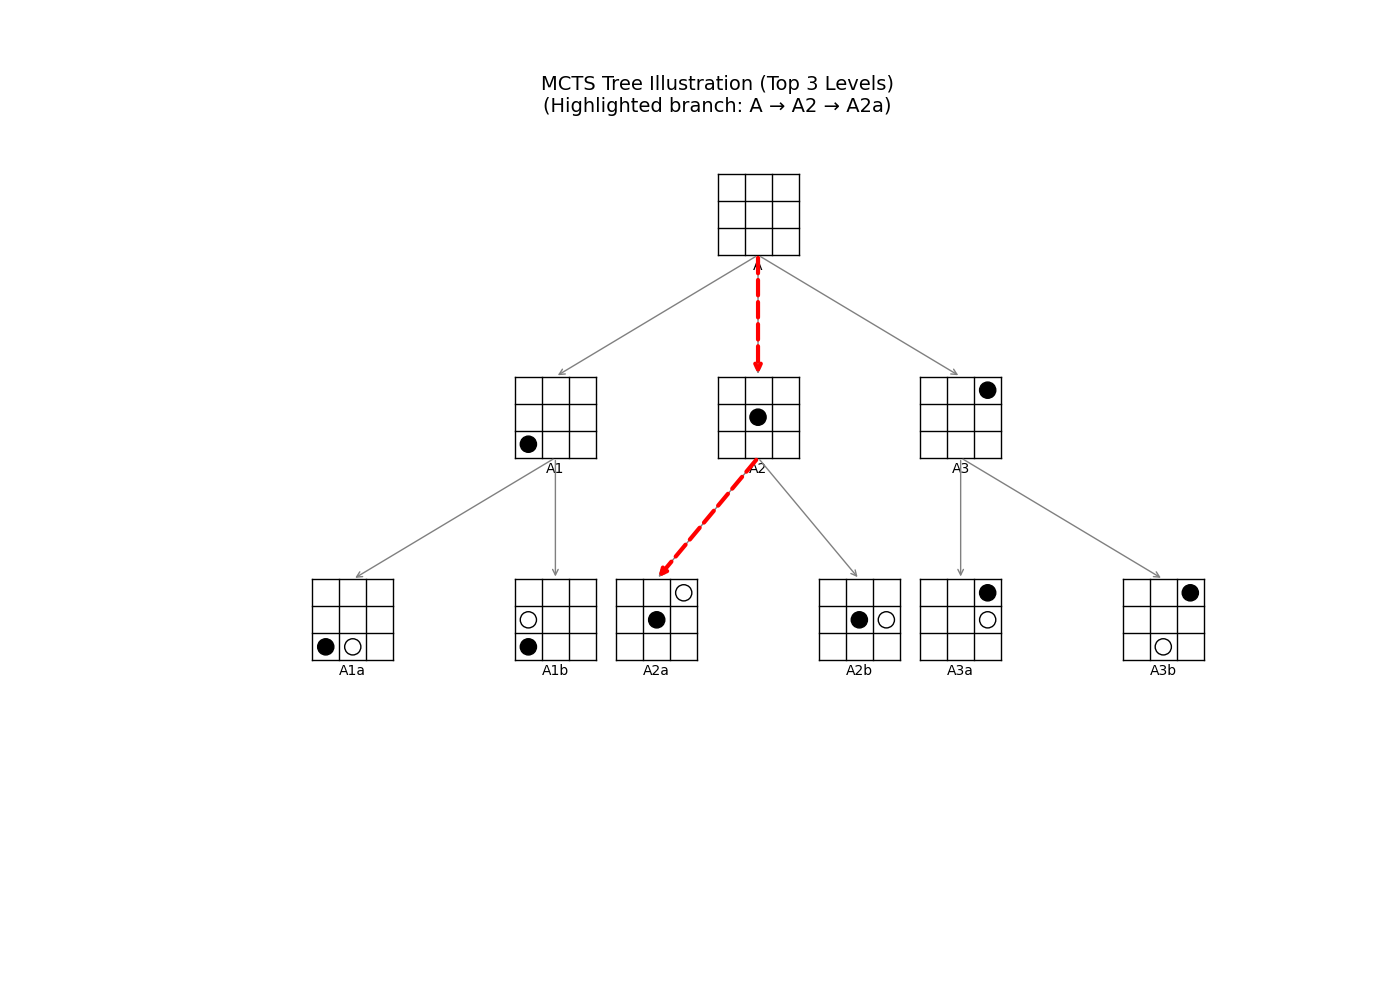
\includegraphics[width=\linewidth]{alpha_go_1.png}

\column{0.50\textwidth}
\centering
\begin{tikzpicture}[
    rootn/.style={circle, draw=RedTitle, fill=blue!10, thick, minimum size=0.55cm, inner sep=0pt, font=\scriptsize},
    childn/.style={circle, draw=gray!60!black, fill=gray!15, thick, minimum size=0.5cm, inner sep=0pt, font=\scriptsize},
    leafn/.style={rectangle, draw=green!50!black, fill=green!15, thick, minimum size=0.35cm, inner sep=1pt, font=\tiny}
]
\node[rootn] (r) at (0,0) {$s$};
\node[childn] (a1) at (-2.4,-1.1) {$a_1$};
\node[childn] (a2) at (-0.8,-1.1) {$a_2$};
\node[childn] (a3) at (0.8,-1.1) {$a_3$};
\node[childn] (a4) at (2.4,-1.1) {$a_4$};

\draw[->] (r) -- (a1);
\draw[->, red!70!black, thick] (r) -- node[font=\tiny, right=2pt, pos=0.5]{$\alpha\sqrt{\tfrac{\ln N(s)}{N(s,a_2)}}$} (a2);
\draw[->] (r) -- (a3);
\draw[->] (r) -- (a4);

\node[leafn] (l1a) at (-2.7,-2.2) {$\hat{V}{=}0.4$};
\node[leafn] (l1b) at (-2.1,-2.2) {$0.5$};
\node[leafn] (l2a) at (-1.1,-2.2) {$0.7$};
\node[leafn] (l2b) at (-0.5,-2.2) {$0.8$};
\node[leafn] (l3a) at (0.5,-2.2) {$0.3$};
\node[leafn] (l3b) at (1.1,-2.2) {$0.2$};
\node[leafn] (l4a) at (2.1,-2.2) {$0.6$};
\node[leafn] (l4b) at (2.7,-2.2) {$0.4$};

\draw[-] (a1) -- (l1a); \draw[-] (a1) -- (l1b);
\draw[-] (a2) -- (l2a); \draw[-] (a2) -- (l2b);
\draw[-] (a3) -- (l3a); \draw[-] (a3) -- (l3b);
\draw[-] (a4) -- (l4a); \draw[-] (a4) -- (l4b);
\end{tikzpicture}

\footnotesize
\textit{Selection $\to$ rollout $\to$ backup.} Same UCB logic as T2; deeper search for higher value.
\end{columns}
\end{frame}

\begin{frame}{Monte Carlo Tree Search: Connection to Economics}
\begin{itemize}
    \item \textbf{MCTS} evaluates moves by simulating future game progressions (\emph{rollouts}).
    \item Four steps: \textbf{Selection} (UCB) $\to$ \textbf{Simulation} (rollout) $\to$ \textbf{Backpropagation} $\to$ \textbf{Move selection}.
\end{itemize}

\vspace{0.3cm}
\textbf{MCTS vs.\ DP:}
\begin{itemize}
    \item DP enumerates \textbf{all} states and transitions.
    \item MCTS selectively simulates \textbf{promising branches}.
    \item Both update value estimates from future returns (Bellman-like).
    \item Key difference: MCTS works when $P(s'|s,a)$ is \textbf{not fully known}.
\end{itemize}

\vspace{0.3cm}
\textbf{For economists:} MCTS is like running targeted ``what-if'' simulations of policy scenarios, focusing computational effort on the most relevant paths through the economy.
\end{frame}


%=============================================================================
% FullCourse-only section: AlphaManager case study (Campello-Cong-Zhou 2023)
% This three-frame case study is unique to FullCourse; MiniCourse has nothing analogous.
\section{Case Study: AlphaManager}

\sectiondivider{Case Study --- AlphaManager}{Offline RL for corporate finance: Campello, Cong \& Zhou (2023)}

\begin{frame}{AlphaManager: Offline RL for Corporate Finance}
\hfill\footnotesize{Campello, Cong \& Zhou (2023), working paper, ``AlphaManager: A Data-Driven-Robust-Control Approach to Corporate Finance''}\normalsize

\textbf{Campello, Cong \& Zhou (2023)} develop an AI-assisted framework (DDRC) for corporate finance:

\vspace{0.3cm}
\textbf{Three challenges addressed:}
\begin{itemize}
    \item \textbf{Curse of dimensionality:} managers' decisions in high-dimensional action/state space.
    \item \textbf{Dynamic feedback:} decisions interact with the economic environment; market reactions feed back.
    \item \textbf{Evolving environment:} data distributions shift as markets evolve.
\end{itemize}

\vspace{0.3cm}
\textbf{Solution approach:}
\begin{enumerate}
    \item \textbf{Predictive Environment Module (PEM):} estimate $\Delta X_{t+1} = f(X_t, u_t) + \varepsilon_{t+1}$ from historical data using deep neural networks.
    \item \textbf{Policy Module:} offline RL (policy gradient) to find optimal $g(X_t|\theta)$.
    \item \textbf{Ambiguity aversion:} penalize actions where model ensemble disagrees, addressing distribution shift.
\end{enumerate}
\end{frame}

\begin{frame}{AlphaManager: Policy Gradient and Ambiguity}
\textbf{Optimization:}
\[
\max_{g(X_t|\theta)} \mathbb{E}_{t_0}\sum_{t=t_0}^{t_0+T} r(X_t, u_t)
\quad \text{s.t.} \quad
\Delta X_{t+1} = f(X_t, u_t) + \varepsilon_{t+1},\; u_t = g(X_t|\theta).
\]

\vspace{0.2cm}
\textbf{Ambiguity via Boosting:}
\begin{itemize}
    \item Train ensemble $\{f^i\}_{i=1}^I$ with different initializations.
    \item Measure disagreement: $\text{BoostingError}(X_t, u_t)$.
    \item Penalize high-disagreement regions:
    \[
    \sum_t \min_i r^i - \delta \cdot \max\{0, \max_t \text{BoostingError} - \theta(X_{t_0})\}.
    \]
\end{itemize}

\vspace{0.2cm}
\textbf{Key insight:} When $\delta \to \infty$, the agent becomes infinitely ambiguity-averse --- it avoids novel, uncertain regions. Balancing $\delta$ is analogous to the exploration--exploitation tradeoff.
\end{frame}

% FullCourse-only: AlphaManager deep dive — added Phase 3.3
\begin{frame}{AlphaManager: Data, Robustness, Consistency Discipline}
\footnotesize
\textbf{Data sources} (offline, observational --- no environment to interact with):
\begin{itemize}
    \item \textbf{BoardEx} (governance covariates), \textbf{Execucomp} (managerial incentives), \textbf{Compustat} (state $X_t$: leverage, cash, payouts, $\ldots$).
\end{itemize}

\textbf{Policy gradient under model ambiguity:}
\begin{itemize}
    \item Reward $r(X_t, u_t)$ encodes the corporate objective (e.g., long-run firm value).
    \item Ambiguity penalty $\delta$ makes the policy \textbf{robust} to misspecified $f$ and $r$.
    \item Closely related to \textbf{robust control} (Hansen \& Sargent) --- familiar territory.
\end{itemize}

\textbf{Three consistency checks} that turn offline RL into a credibility-bearing artifact:
\begin{enumerate}
    \item \textbf{Cross-validation:} hold-out \emph{firms} --- guards against firm-FE leakage.
    \item \textbf{Out-of-sample:} hold-out \emph{years} --- guards against regime drift (pre/post-GFC).
    \item \textbf{Interpretability subsamples:} actions on regulator-friendly slices (small / leveraged firms) checked against domain expectations.
\end{enumerate}

\textit{The same triangulation logic resurfaces in Lec09 T5 on agent-assisted research --- multi-agent debate as a consistency check on LLM-generated economic reasoning.}
\normalsize
\end{frame}

\begin{frame}{AlphaManager: Consistency and Extensions}
\textbf{Consistency question:}
\begin{itemize}
    \item PEM estimates $f(X_t, u_t)$ from historical data.
    \item Optimal policy $g^*$ (given $f$) changes behavior $\Rightarrow$ new data distribution.
    \item Will the estimated $f$ remain valid under the new policy?
\end{itemize}

\vspace{0.15cm}
\textbf{Possible extension --- toward full RL:}
\begin{enumerate}
    \item Use solved $g(X|f)$ to generate new data via bootstrap.
    \item Mix new (out-of-sample) data with historical data.
    \item Re-estimate $\hat{f}$ with a learning rate for new observations; repeat until $f$ and $\hat{f}$ converge.
\end{enumerate}

\vspace{0.1cm}
This moves from \textbf{offline RL} (fixed dataset) toward \textbf{online RL} (iterative environment learning) --- improving robustness and discovering strategies invisible in historical data alone.

\vspace{0.1cm}
\footnotesize\textit{Forward pointer:} Lec09 T5 returns to consistency mechanisms in agent-assisted research --- Du et al.\ (2023) on multi-agent debate; Irving, Christiano \& Amodei (2018) on AI safety via debate. AlphaManager's checks are a domain-specific instance.\normalsize
\end{frame}


%=============================================================================
% NEW: Krusell-Smith deep actor-critic application (book Ch13 §7) --- final economic application
\section{Application: Krusell--Smith via Deep RL}

\sectiondivider{Application --- Krusell--Smith via Deep RL}{The heterogeneous-agent workhorse, solved with a deep actor--critic (the bridge to Lec06)}

\begin{frame}{Application: Krusell--Smith with Deep Actor-Critic}
\hfill\footnotesize{Krusell \& Smith (1998); Feng, Han, Sargent \& Zhu (2025)}\normalsize

\textbf{The hard part:} in a heterogeneous-agent model the \textbf{wealth distribution $\Phi$ is a state} --- infinite-dimensional, and its law of motion $\Phi'=\mathcal{T}(\Phi)$ has no closed form.
\begin{itemize}
  \item \textbf{Histogram representation:} bin assets into shares $\widehat f_a = [x_1,\dots,x_N]$, $\sum_i x_i = 1$ --- a finite vector a neural net can read.
  \item \textbf{Actor} $\pi_\theta(a'\,|\,a,z,Z,\widehat f_a)$ = household savings policy; \textbf{Critic} $V_w(\cdot)$ = household value.
  \item \textbf{Prices clear internally:} $K=\sum_i x_i\bar a_i \Rightarrow (r,w)$ from the firm's FOCs each period --- no external forecast-rule iteration (the KS shortcut).
\end{itemize}
\end{frame}

\begin{frame}{Krusell--Smith: Why Deep Actor-Critic Scales}
\textbf{Three properties tame the dimensionality:}
\begin{itemize}
  \item NN first-layer parameters grow \textbf{linearly} in the input dimension (not $m^d$).
  \item Monte-Carlo simulation concentrates samples on the \textbf{ergodic set} --- where households actually are.
  \item The neural critic gives \textbf{grid-free} interpolation over the simulated ``point cloud.''
\end{itemize}
\vspace{0.15cm}
\begin{conceptbox}
The AlphaGo lesson, applied to macro: \emph{neural value$+$policy approximation $+$ sampling} reaches models classical grid-based DP cannot --- but the curse is \textbf{mitigated, not eradicated}, and credibility still rests on the calibrated model.
\end{conceptbox}
\end{frame}


%=============================================================================
\section{Summary}

\sectiondivider{Summary}{Three acts, one backbone --- and the one caveat that keeps it credible}

\begin{frame}{Lecture Summary}
\begin{enumerate}
    \item \textbf{RL = DP + Learning}: same Bellman foundations, but replaces full expectation backup with \textbf{sample-based} updates.

    \item \textbf{Monte Carlo}: learns from complete episodes; model-free but slow and high-variance.

    \item \textbf{TD / Q-Learning}: incremental updates after each step; balances bias and variance; handles continuing tasks.

    \item \textbf{Actor-Critic}: combines policy optimization (actor) with value estimation (critic); handles continuous actions and large state spaces.

    \item \textbf{Advanced algorithms} (PPO, SAC, DDPG): stability, entropy regularization, deterministic policies for different use cases.

    \item \textbf{For economists}: RL enables solving dynamic models that are too high-dimensional for classical DP, and environments where transition probabilities are unknown or endogenous.
\end{enumerate}
\end{frame}

%=============================================================================
% All-done MAP reprise (mirrors Lec09 T5's closing reprise): three acts complete.
\begin{frame}{The Whole Lecture in One Map}
\textbf{Three acts, one backbone. The Bellman / GPI skeleton never changed --- only \emph{how we filled the expectation} did.}

\LecFiveMap{0}

\vspace{0.05cm}
\footnotesize\textit{\textbf{5.1 MODEL}: known $P,R$ $\Rightarrow$ full backup (classical DP). \quad \textbf{5.2 SAMPLE}: no model $\Rightarrow$ sample backup (MC, TD, Q-learning). \quad \textbf{5.3 SCALE}: sampled $+$ function-approximated $\Rightarrow$ deep RL (actor--critic, DQN) for continuous, high-dimensional economies.}
\end{frame}


% NEW: Part-3 synthesis --- what economists can borrow + the caveat
\begin{frame}{What Economists Can Borrow from RL --- and the One Caveat}
\small
\textbf{One skeleton, two ways to fill the expectation.} DP and RL share the Bellman/GPI backbone; DP is RL's \emph{structural} special case (known $P$, small $|\mathcal{S}|$). So we \textbf{extend} DP, not abandon it --- and RL is \emph{not} merely a last resort (``deep DP'' helps even when $P$ is known).
\begin{itemize}
  \item \textbf{Sample backup} $\to$ solve high-dimensional / distribution-valued models.
  \item \textbf{Function approximation} $\to$ scale (a \emph{shared} tool; the threat is the deadly triad).
  \item \textbf{Actor-critic} $\to$ the online two-step / GMM estimator economists already know.
  \item \textbf{Off-policy $+$ importance sampling} $\to$ counterfactual policy evaluation (coverage $=$ overlap).
\end{itemize}
\normalsize
\begin{takeawaybox}
\footnotesize \textbf{The caveat that makes it principled:} \emph{RL scales the solution, not the identification.} Train in a calibrated structural model, validate out of sample. ``Isn't RL just DP plus sampling?'' --- yes in \emph{structure}; no in \emph{reach} (the information and computation dimensions).\normalsize
\end{takeawaybox}
\end{frame}

\begin{frame}{The RL Landscape for Economists}
\centering
\begin{tabular}{lcc}
\toprule
\textbf{Method} & \textbf{Model Required?} & \textbf{Update Style} \\
\midrule
Value Function Iteration (DP) & Yes (full model) & Full backup \\
Monte Carlo & No & End of episode \\
TD(0) / SARSA & No & Every step \\
Q-Learning & No & Every step (off-policy) \\
Actor-Critic & No & Every step (policy + value) \\
\midrule
\textbf{Deep RL variants} & & \\
DQN / DDPG / PPO / SAC & No & Mini-batch gradient \\
\bottomrule
\end{tabular}

\vspace{0.5cm}
\textbf{As models grow in complexity, RL becomes not a replacement for DP, but its necessary \textbf{generalization}.}
\end{frame}


% FullCourse-only: Key Takeaways recap frame (Mini stops at Topic 2.3 Recap)
\begin{frame}{Key Takeaways}
\begin{itemize}
    \item Economists already know the theory behind RL --- it's the \textbf{Bellman equation}.
    \item What RL adds: the ability to \textbf{learn} value functions and policies from \textbf{simulated experience} rather than solving them analytically.
    \item The exploration--exploitation tradeoff has direct economic interpretations (R\&D, pricing, portfolio choice).
    \item Actor-critic methods are the workhorse for solving continuous-action dynamic models with deep learning.
    \item Modern breakthroughs (AlphaGo, RLHF for LLMs) rest on the same foundations covered today.
\end{itemize}

\vspace{0.3cm}
\begin{takeawaybox}
\footnotesize \textbf{The one caveat that keeps it credible:} RL scales the \emph{solution}, not the \emph{identification}. Train inside a calibrated structural model, validate out of sample --- RL's credibility inherits the model's.
\end{takeawaybox}
\end{frame}

% FullCourse-only: Lec06 forward bridge --- the deck's closing hand-off.
\begin{frame}{Bridge to Lec06: The Toolkit Doesn't Change --- the State Space Does}
\textbf{Act 5.3 scaled RL from tables to neural networks. Lec06 turns exactly this machinery onto heterogeneous-agent models that were intractable a decade ago.}

\vspace{0.15cm}
\begin{itemize}
    \item \textbf{Lec06 T1 --- Aiyagari computation:} the canonical HA workhorse gets the RL treatment; classical projection $+$ iteration vs.\ DNN-based global solvers.
    \item \textbf{Lec06 T2 --- Why ML for HA $+$ global DNN:} Euler-equation training as a direct application of value/policy nets (Lec04 T3) at HA scale.
    \item \textbf{Lec06 T3 --- Krusell--Smith via DeepHAM:} deep value-and-policy learning --- the actor--critic family of Act 5.3 at high-dimensional aggregate states (Han, Yang \& E, 2021; \emph{Quantitative Economics} 2026).
    \item \textbf{Lec06 T4 --- Deep Equilibrium Nets (DEQN) $+$ OLG} with aggregate uncertainty (Azinovic, Gaegauf \& Scheidegger, 2022).
    \item \textbf{Lec06 T5 --- Mean-Field Games (HJB $+$ KFE):} RL for the continuum-of-agents limit.
\end{itemize}

\vspace{0.1cm}
\begin{center}
\footnotesize\textit{Hands-on (Session-4 lab): you build one of these deep HA solvers yourself --- Krusell--Smith (1998) via Deep Equilibrium Nets in PyTorch.}\\[2pt]
\footnotesize\textit{Arc complete: 5.1 MODEL $\;\to\;$ 5.2 SAMPLE $\;\to\;$ \textbf{5.3 SCALE} $\;\Longrightarrow\;$ \textbf{Lec06}: heterogeneous agents at scale.}
\end{center}
\end{frame}

\end{document}
